\item \textbf{{[}HCI/PRELIM/9569/2021/P1/Q7{]}}
\begin{enumerate}
\item {}
\begin{enumerate}
\item What is a flowchart? \hfill{}{[}1{]}
\item Draw a flowchart to find the factorial of a given positive integer
\texttt{N}.\hfill{} {[}2{]}
\end{enumerate}
\item You have a row of \texttt{2}n disks of two colors, \texttt{n} black
and \texttt{n} white. They alternate: black, white, black, white,
and so on. You want to get all the black disks to the right-hand end,
and all the white disks to the left-hand end. The only moves you are
allowed to make are those that interchange the positions of two neighboring
disks.
\begin{center}
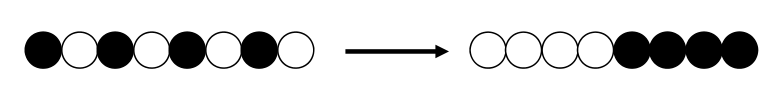
\includegraphics[width=0.5\paperwidth]{C:/Users/Admin/Desktop/Github/question_bank/LyX/static/img/9569-HCI-2021-P1-Q7}
\par\end{center}

Assume that there is an array \texttt{A} of size \texttt{2n} representing
the alternating disks. Write, in \textbf{pseudocode}, an algorithm
to solve this puzzle and determine the number of moves it takes. \hfill{}{[}5{]}
\end{enumerate}